\documentclass{article}

\usepackage{amsmath}
\usepackage{amssymb}
\usepackage{amsthm}
\usepackage{bm}
\usepackage{tikz}
\usetikzlibrary{positioning}

\begin{document}
    \newcommand\norm[1]{\left\lVert#1\right\rVert}
    

    % Define the x-offset as a variable
    \newcommand{\xoffset}{0.0}

    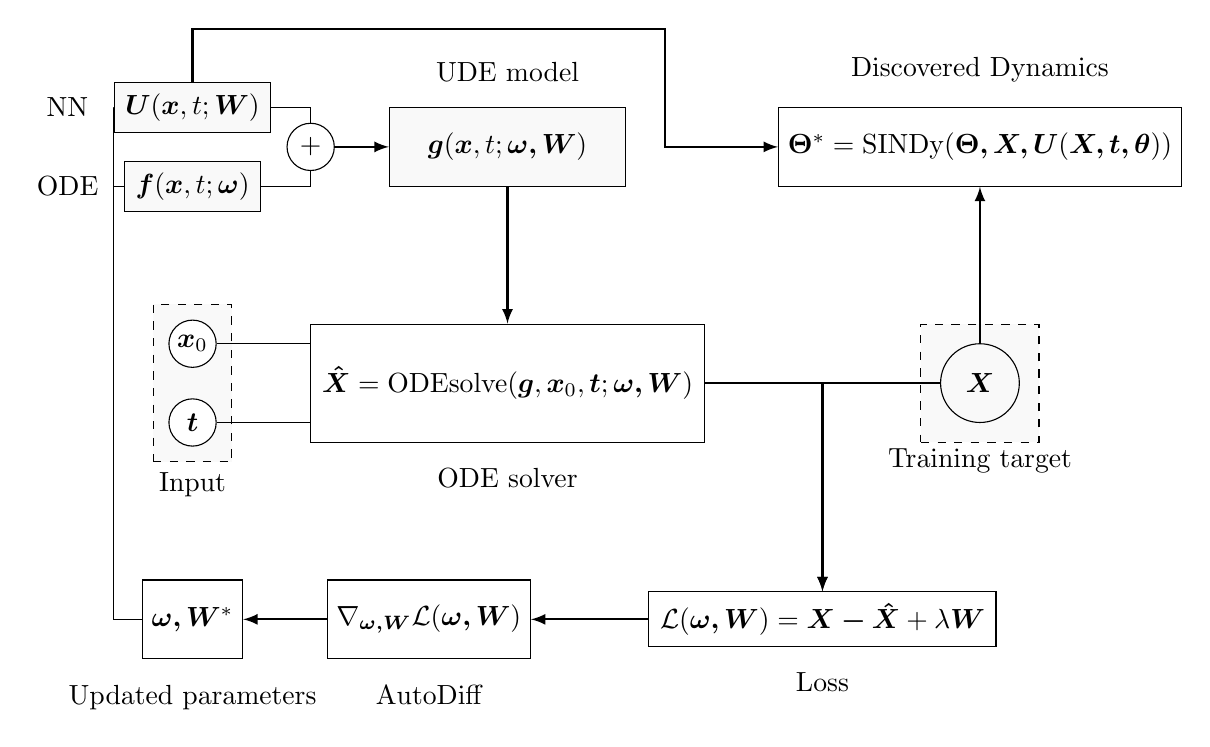
\begin{tikzpicture}[
        neuron/.style={rectangle, inner sep=4.0 },
        bias/.style={circle, draw, minimum size=0.8cm, fill=darkgray, inner sep=0},
        weight/.style={circle, draw, minimum size=0.6cm, fill=white, inner sep=0},
        line/.style={-latex, thick}
    ]

    % Layer 1

    %dashed rectangle
    \node[rectangle,draw, dashed, minimum width=1cm, minimum height=2.cm,fill=gray!5, align=center] at (0, 0.5) {}; 
    \node[weight] (t) at (0, 0) {$\bm{t}$};
    \node[weight] (x) at (0, 1) {$\bm{x}_0$};
    \node[below=0.2cm of t] {Input};
    

    \node[neuron, draw,fill = gray!5] (ode) at (0, 3) {$\bm{f}(\bm{x}, t; \bm{\omega})$};
    \node[left=0.2cm of ode] {ODE};

    \node[neuron, draw, fill = gray!5] (NN) at (0, 4) {$\bm{U}(\bm{x}, t; \bm{W})$};
    \node[left=0.2cm of NN] {NN};
    
    \node[weight] (add) at (1.5, 3.5) {$+$};
    
    %Layer 2
    \node[rectangle,draw, minimum width=3cm, minimum height=1cm,fill=gray!5, align=center] 
        (model) at (4, 3.5) {$\bm{g}(\bm{x}, t; \bm{\omega, W})$};
    \node[above=0.2cm of model] {UDE model};
    
    \node[neuron, draw, align=center, minimum height =1.5cm] 
        (ODEsolver) at (4, 0.5) {$\bm{\hat{X}}= \text{ODEsolve}(\bm{g}, \bm{x}_0, \bm{t}; \bm{\omega, W})$};
    \node[below=0.2cm of ODEsolver] {ODE solver};
    
    %Layer 3
    \node[neuron, draw]
        (Loss) at (8, -2.5) {$\mathcal{L}(\bm{\omega, W})= \norm{\bm{X- \hat{X}}} + \lambda \norm{\bm{W}}$};
    \node[below=0.2cm of Loss] {Loss};


    %Layer 4
    \node[rectangle,draw, dashed, minimum width=1.5cm, minimum height=1.5cm,fill=gray!5, align=center] at (10,0.5) {}; 
    \node[circle, draw, align=center, minimum width=1cm, minimum height=1cm]
        (training target) at (10, 0.5) {$\bm{X}$};
    \node[below=0.2cm of training target] {Training target};    

    %bottom
    \node[rectangle, draw, align=center, minimum width=1cm, minimum height=1cm] 
        (gradient) at (3, -2.5) {$\nabla_{\bm{\omega, W}} \mathcal{L}(\bm{\omega, W})$};
    \node[below=0.2cm of gradient] {AutoDiff};

        
    \node[rectangle, draw, align=center, minimum width=1cm, minimum height=1cm] 
        (converged) at (0, -2.5) {$\bm{\omega, W}^*$};
    \node[below=0.2cm of converged] {Updated parameters};

    

    %SINDy
    \node[rectangle, draw, align=center, minimum width=1cm, minimum height=1cm] 
        (sindy) at (10, 3.5) {$\bm{\Theta }^* = \text{SINDy}(\bm{\Theta,X, U}(\bm{X, t, \theta}))$};
    \node[above=0.2cm of sindy] {Discovered Dynamics};

    
    % Arrows without arrowhead
    % Layer 1 to Layer 2
    \draw (ode) -| (add);
    \draw (NN) -| (add);
    \draw[line] (add) -- (model);
    \draw (x) -| (ODEsolver.west);
    \draw (t) -| (ODEsolver.west);


    \draw[line] (model) -- (ODEsolver);
    \draw[line] (ODEsolver) -| (Loss);

    \draw[line] (training target) -| (Loss);
    % bottom layer
    \draw[line] (Loss) -- (gradient);
    \draw[line] (gradient) -- (converged);

    \draw (converged) --++(-1, 0.) |- (ode.west);
    \draw (converged) --++(-1,.0) |- (NN.west);

    %SINDy
    \draw[line] (training target) -- (sindy);
    \draw[line] (NN) --++(0., 1.0) --++ (6, 0.) |- (sindy.west);
    
    \end{tikzpicture}
\end{document}